\documentclass[12pt]{article}

\usepackage{graphicx}
\usepackage{pdfpages}
\usepackage{listings}
\usepackage{amsmath}
\usepackage{subcaption}
\usepackage{todonotes}
\usepackage{arydshln}

\renewcommand{\figurename}{Fig.}

\title{TTK4210 Advanced Control of Industrial Systems, Exercise 6}
\date{}
\author{Kristian Løvland}

\begin{document}
\maketitle
\tableofcontents

\newpage
\section{Abstract}
In this project, a model of a butane distillation column was used to design a controller for the composition of two product streams consisting of n-butane and iso-butane, respectively. By identifying characteristics of relevant subsystems, PI controllers for the states of these systems were designed with the ultimate goal of keeping the purity of the products at a satisfactory level.

\newpage
\section{Introduction}
A good introduction to the control problem we're faced with is given in the assignment text \cite{oppgavetekst}. A short summary follows

The top product is required to contain no more than 4\% n-butane, while the bottom product is required to contain less than 2,5\% iso-butane. 

These compositions, denoted $x_D^*$ and $x_B^*$ are in practice controlled through their temperatures. These are measured on the top and bottom of the distillation column, and are denoted $T_D$ and $T_B$. The temperature needed to acheive the required compositions are shown in \ref{tab:requirements}, together with the actual temperature setpoint. These are a bit lower/higher than they strictly need to introduce a safety margin.

\begin{table}[h]
\centering
\begin{tabular}{c | c | c }
& Required temperature & Temperature setpoint\\ \hline
Top product ($D$) & $35,85^\circ$ C & $35,30^\circ$ C\\
Bottom product ($B$) & $47,69^\circ$ C & $48,51^\circ$ C
\end{tabular}
\caption{Temperatures giving satisfactory product quality}
\end{table}

To satisfy these specifications, the rest of the systems need to work well too. The levels $M_D$ and in the top accumulator and $M_B$ in the distillation column need to be controlled to stable setpoints. The same goes for distillation column pressure $p$.

To control these five variables, five degrees of freedom is needed. Our five manipulated variables are flow rates in different parts of the system, denoted $V_T$, $L$, $D$, $V$ and $B$. Each of these is controlled directly by a valve. \todo{Sjekk om dette stemmer}

Table \ref{tab:pairings} shows the pairing of manipulated and controlled variables. As mentioned, it is assumed that choosing good setpoints for $T_D$ and $T_B$ gives satisfactory product quality. This control structure is called LV-control, after the manipulated variables used to control product quality.

\begin{table}[h]
\centering
\begin{tabular}{c|ccccc}
Manipulated Variable & $V_T$ & $D$ & $B$ & $L$ & $V$ \\ \hline
Controlled variable & $p$ & $M_D$ & $M_B$ & $T_D$ & $T_B$
\end{tabular}

\caption{Variable pairings}
\label{tab:pairings}
\end{table}

\newpage
\section{Tuning secondary controllers}
The secondary controllers were tuned individually using the SIMC method for PI controllers. A step in process input with an amplitude small enough to not cause problems (usually meaning 50\% of maximum accepted input magnitude) in other parts of the system was used for all the secondary controllers, controlling the states $D$, $L$, $B$, $V$ and $p$.

A summary of the method is given in \cite{regtek}. The method assumes that the system can be approximated by a first order process with time delay

\begin{equation}
G(s) = \frac{k e^{-\theta s}}{1 + T_1 s}
\end{equation}
and be controlled by a PI controller

\begin{equation}
K(s) = K_p\frac{1 + T_i s}{T_i s}
\end{equation}

The SIMC method gives rules for choosing $K_p$ and $T_i$, given a desired closed-loop time contant $T_L$. Assuming the step response behaves similarly to a first order system, the method is then as follows

\begin{enumerate}
\item Fit the step response to a first order model. This means finding time delay $\theta$, slope $k' = \frac{dy/dt}{\Delta u}$ and time constant $T_1$ from the plot of the step response.
\item To achieve the desired time constant $T_L$, use the PI controller parameters $K_p = \frac{1}{k'} \frac{1}{\tau + T_L}$, $T_i = \min(T_1, 4(\tau + T_L))$.
\end{enumerate}

% Figurer, open-loop stegrespons
\begin{figure}[p]
\centering
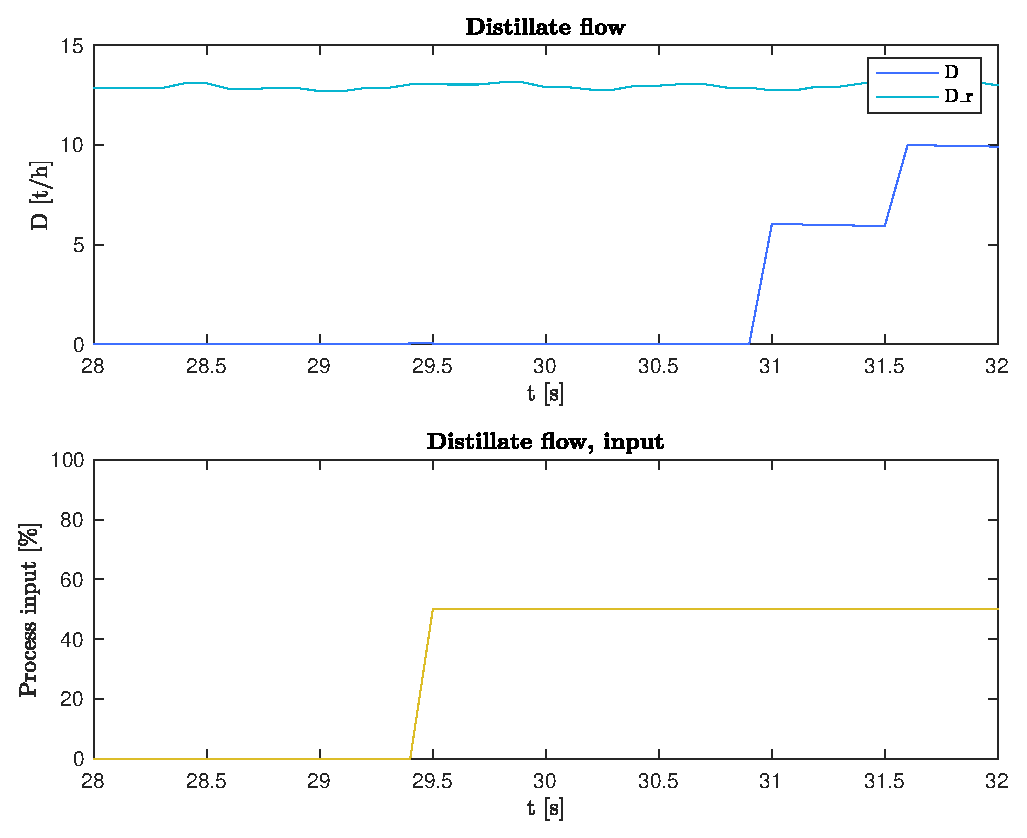
\includegraphics[width=0.8\textwidth]{../Systemanalyse/Log_Data_to_Matlab/Figurer/Stegeksperimenter/FC1005.eps}
\caption{Open-loop step response of $D$}
\label{fig:ol_step_FC1005}

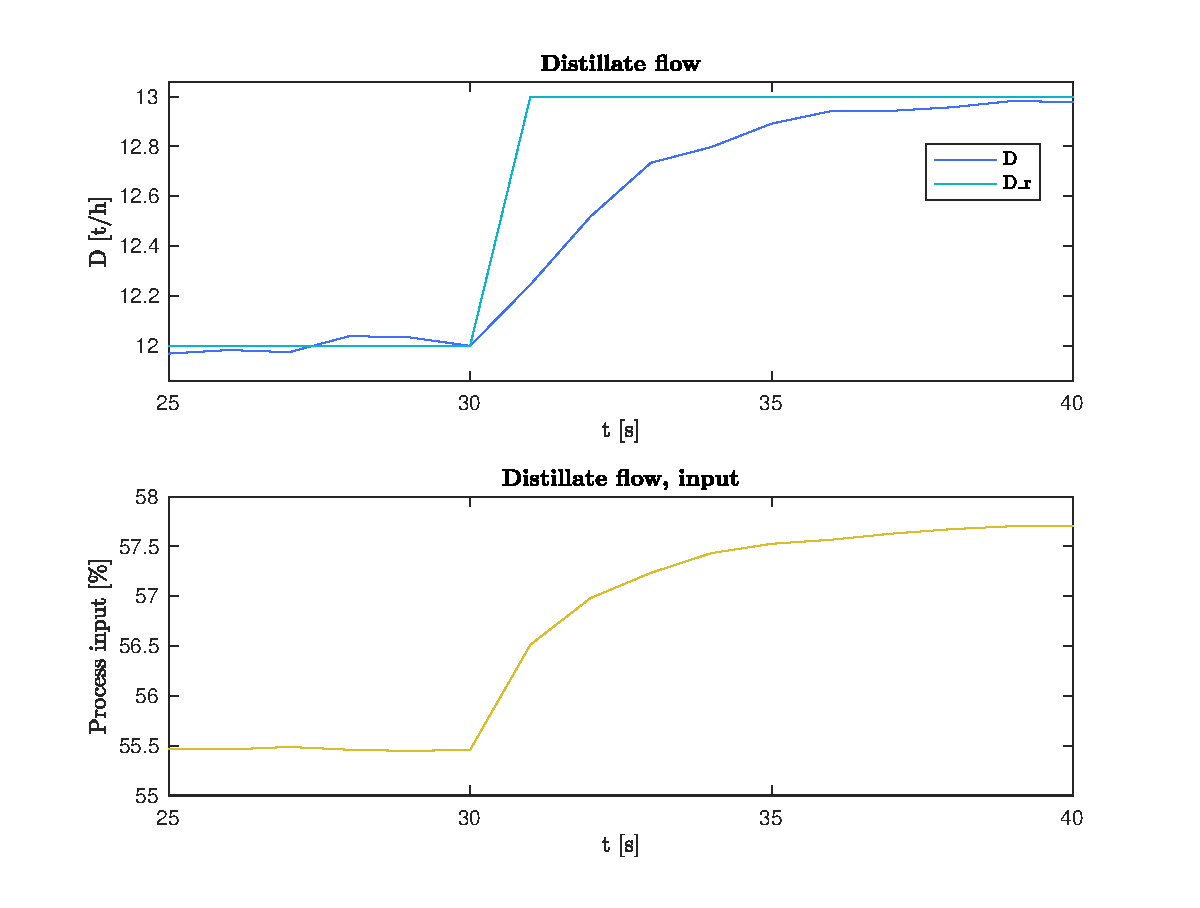
\includegraphics[width=0.8\textwidth]{../Systemanalyse/Log_Data_to_Matlab/Figurer/Stegeksperimenter/FC1005_step.eps}
\caption{Closed-loop step response of $D$}
\label{fig:cl_step_FC1005}
\end{figure}

\begin{figure}[p]
\centering
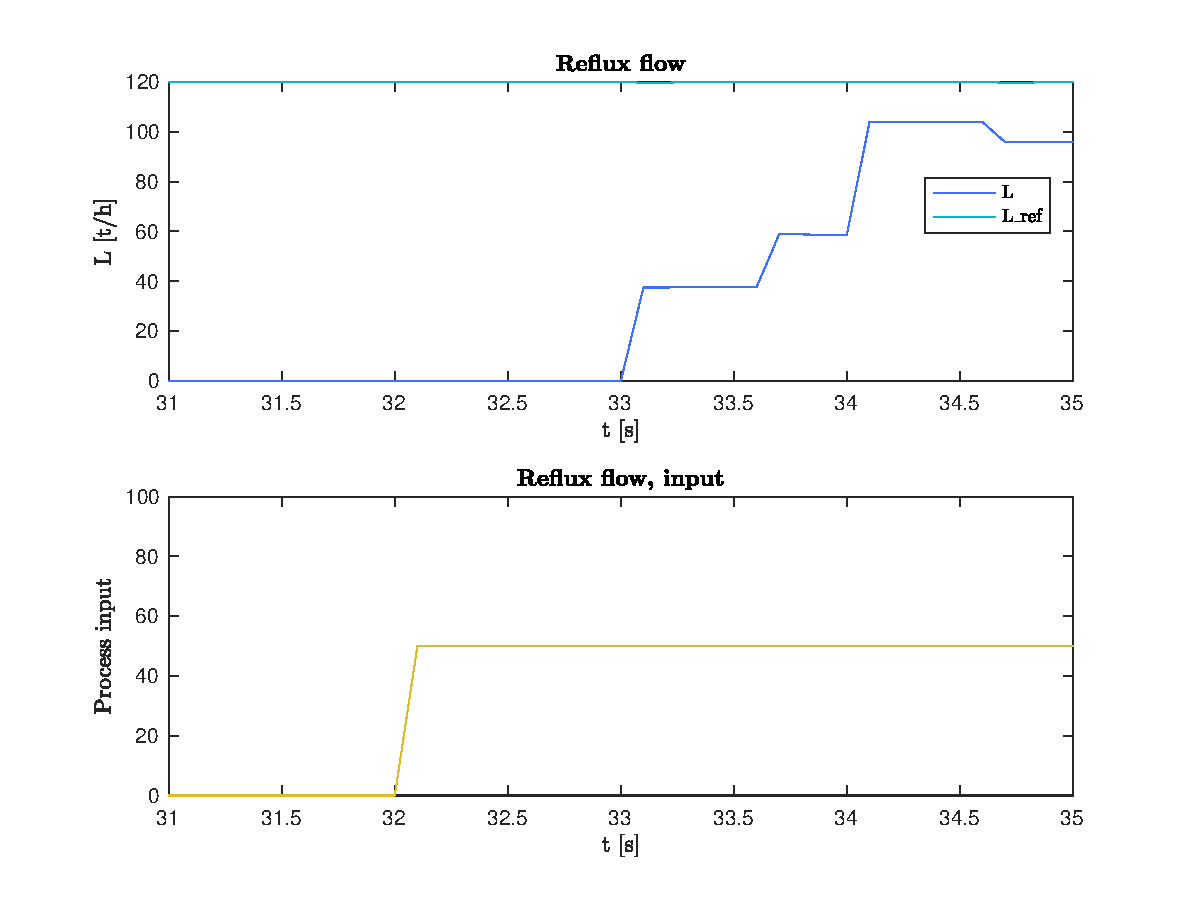
\includegraphics[width=0.8\textwidth]{../Systemanalyse/Log_Data_to_Matlab/Figurer/Stegeksperimenter/FC1015.eps}
\caption{Open-loop step response of $L$}
\label{fig:ol_step_FC1015}

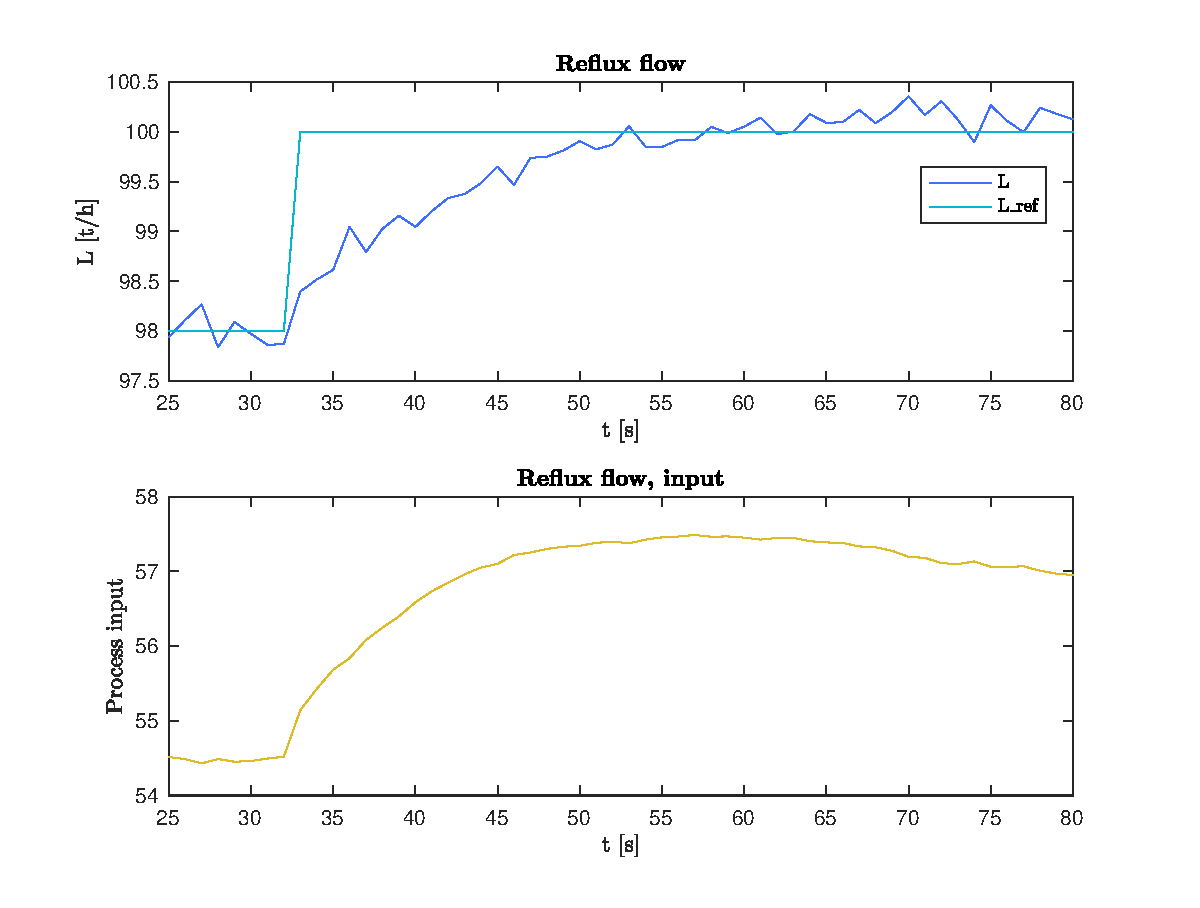
\includegraphics[width=0.8\textwidth]{../Systemanalyse/Log_Data_to_Matlab/Figurer/Stegeksperimenter/FC1015_step.eps}
\caption{Closed-loop step response of $L$}
\label{fig:cl_step_FC1015}
\end{figure}

\begin{figure}[p]
\centering
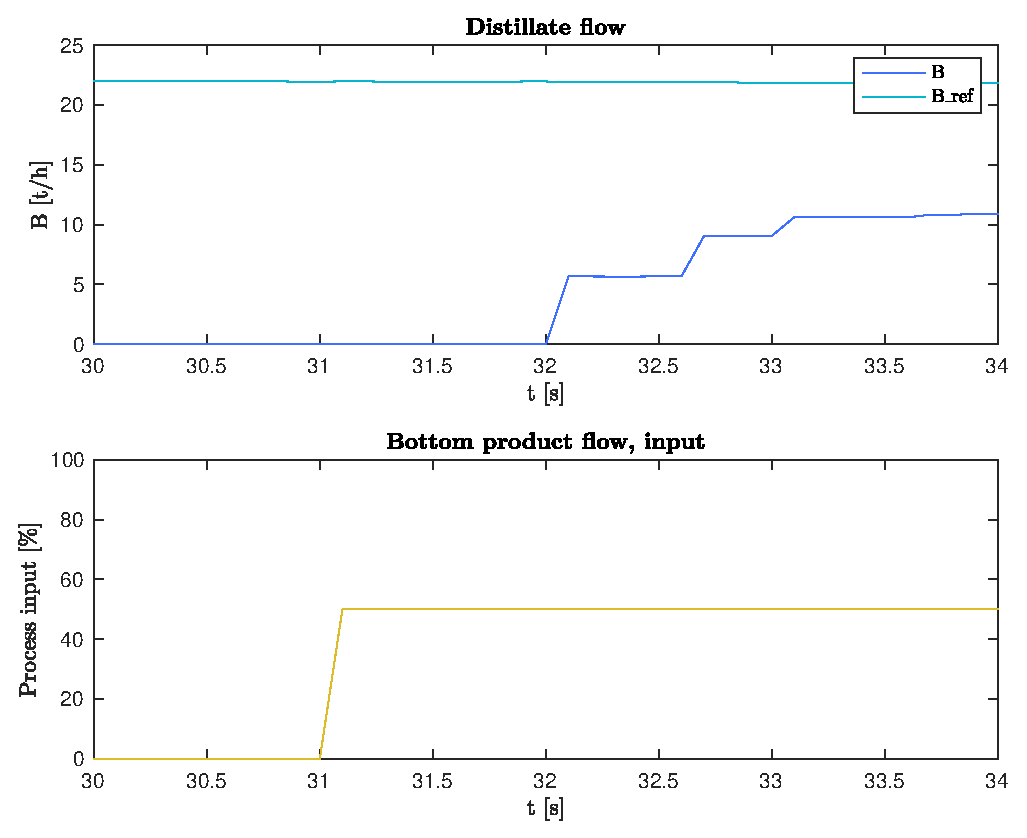
\includegraphics[width=0.8\textwidth]{../Systemanalyse/Log_Data_to_Matlab/Figurer/Stegeksperimenter/FC1019.eps}
\caption{Open-loop step response of $B$}
\label{fig:ol_step_FC1019}

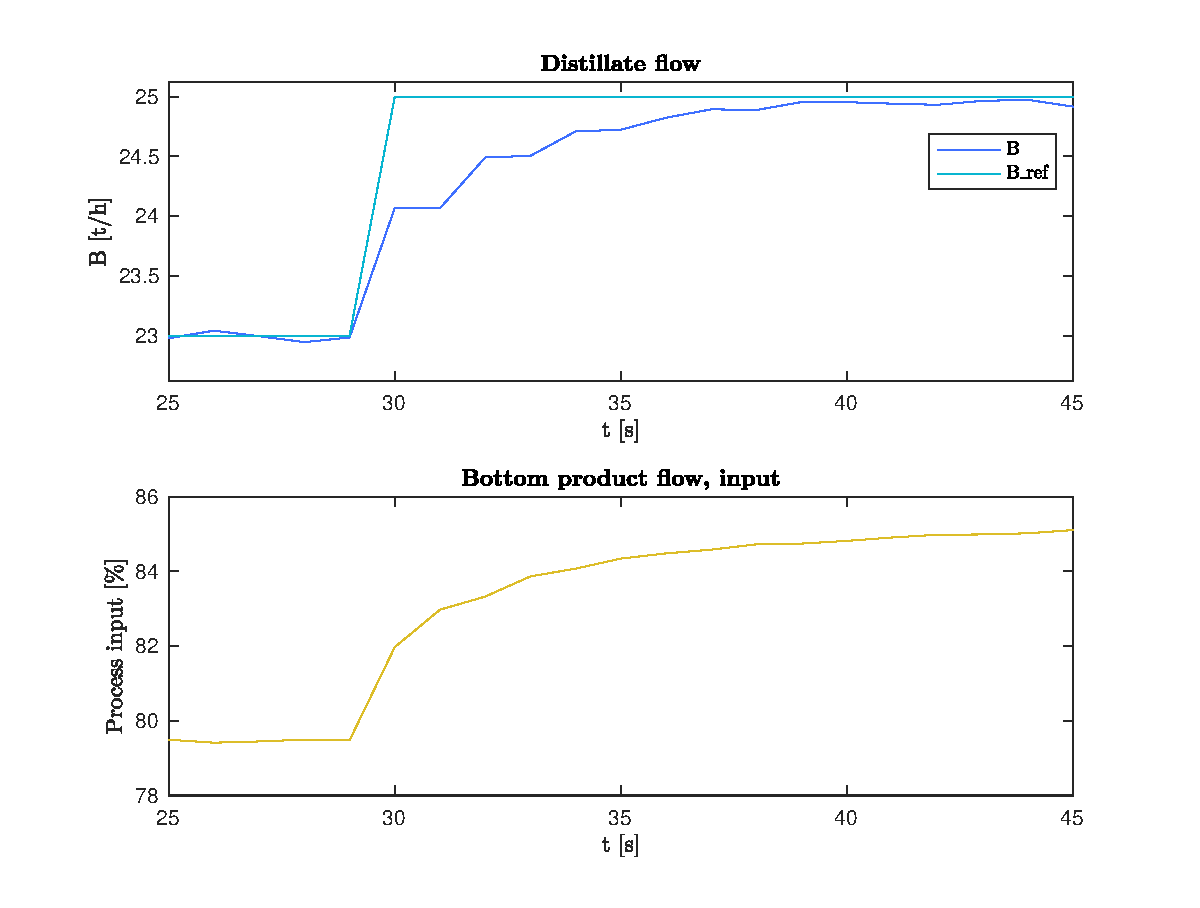
\includegraphics[width=0.8\textwidth]{../Systemanalyse/Log_Data_to_Matlab/Figurer/Stegeksperimenter/FC1019_step.eps}
\caption{Closed-loop step response of $B$}
\label{fig:cl_step_FC1019}
\end{figure}

\begin{figure}[p]
\centering
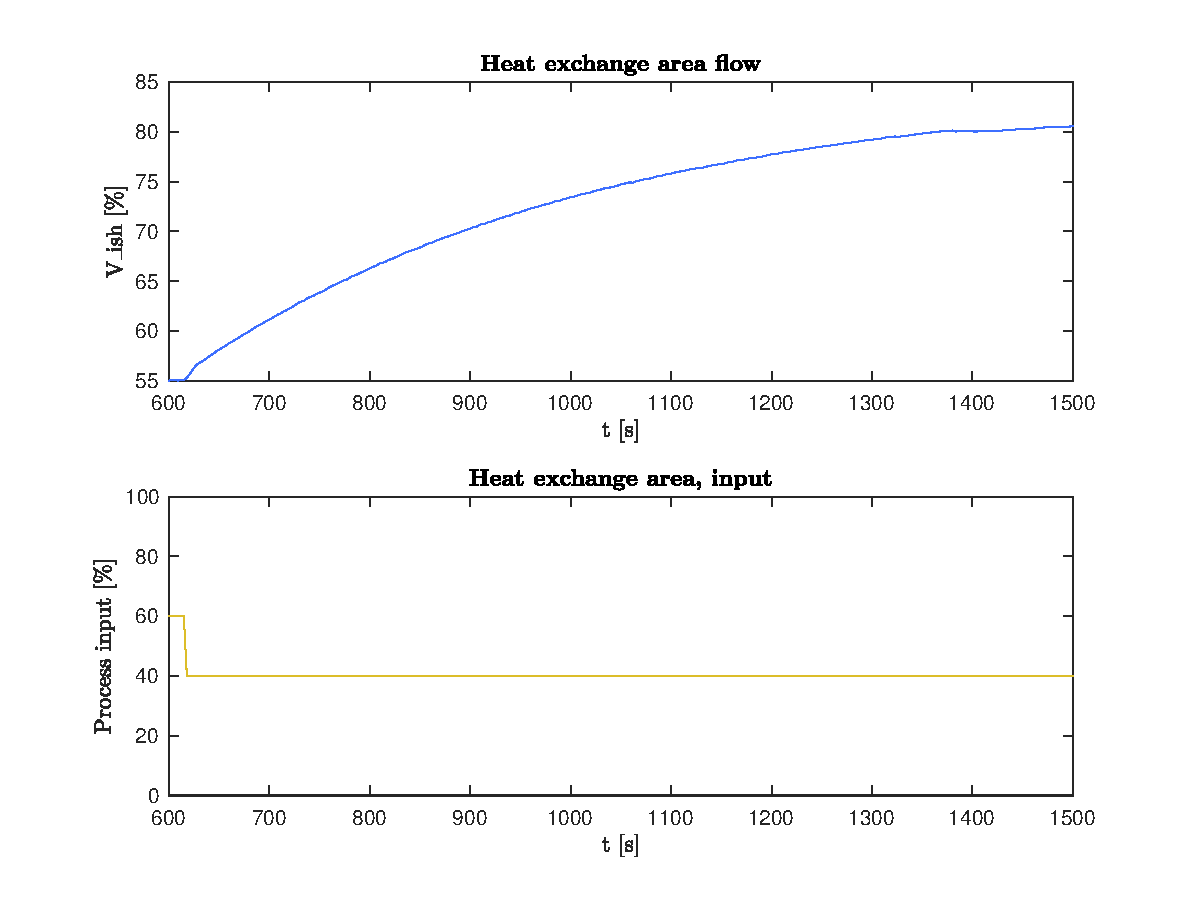
\includegraphics[width=0.8\textwidth]{../Systemanalyse/Log_Data_to_Matlab/Figurer/Stegeksperimenter/LC1028.eps}
\caption{Open-loop step response of heat exchanger area, related to $V$}
\label{fig:ol_step_LC1028}

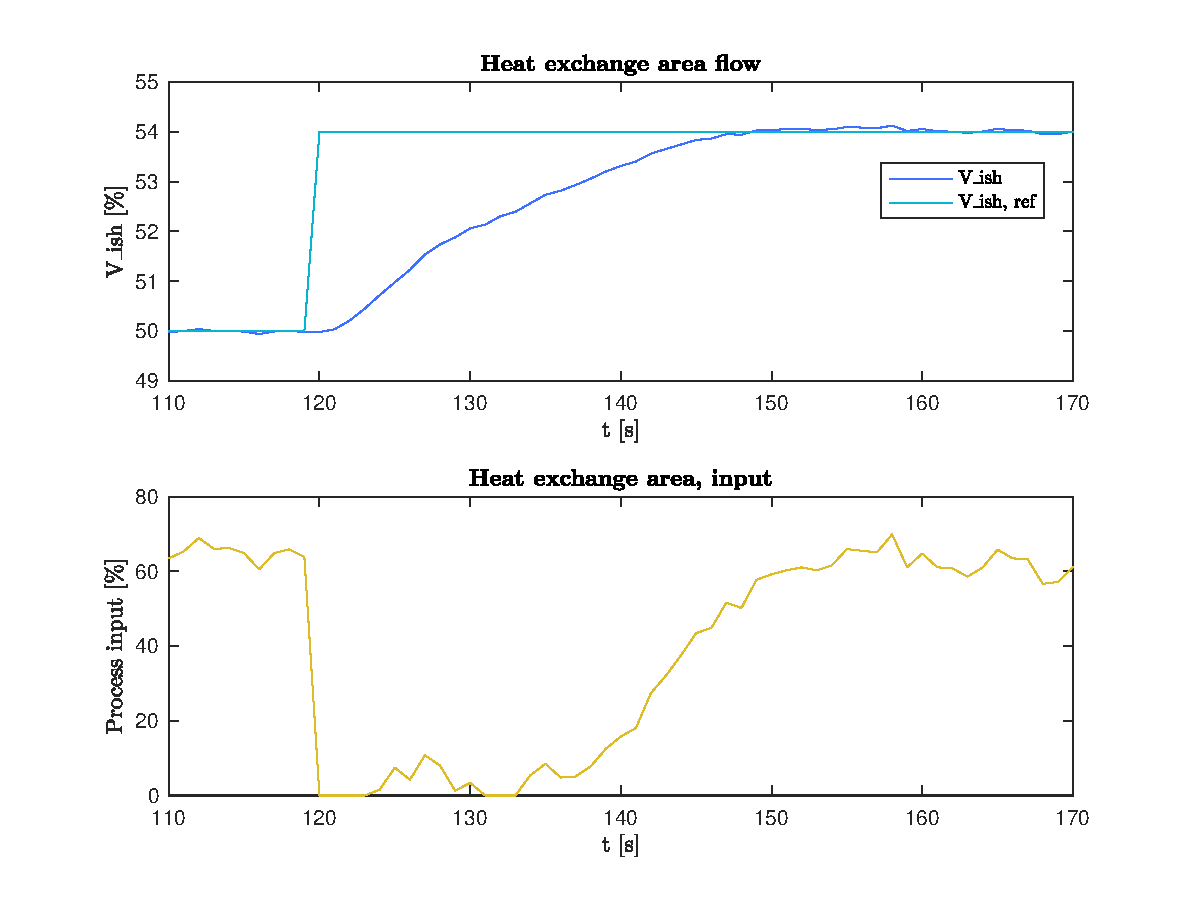
\includegraphics[width=0.8\textwidth]{../Systemanalyse/Log_Data_to_Matlab/Figurer/Stegeksperimenter/LC1028_step.eps}
\caption{Closed-loop step response of heat exchanger area, related to $V$}
\label{fig:cl_step_LC1028}
\end{figure}

\begin{figure}[p]
\centering
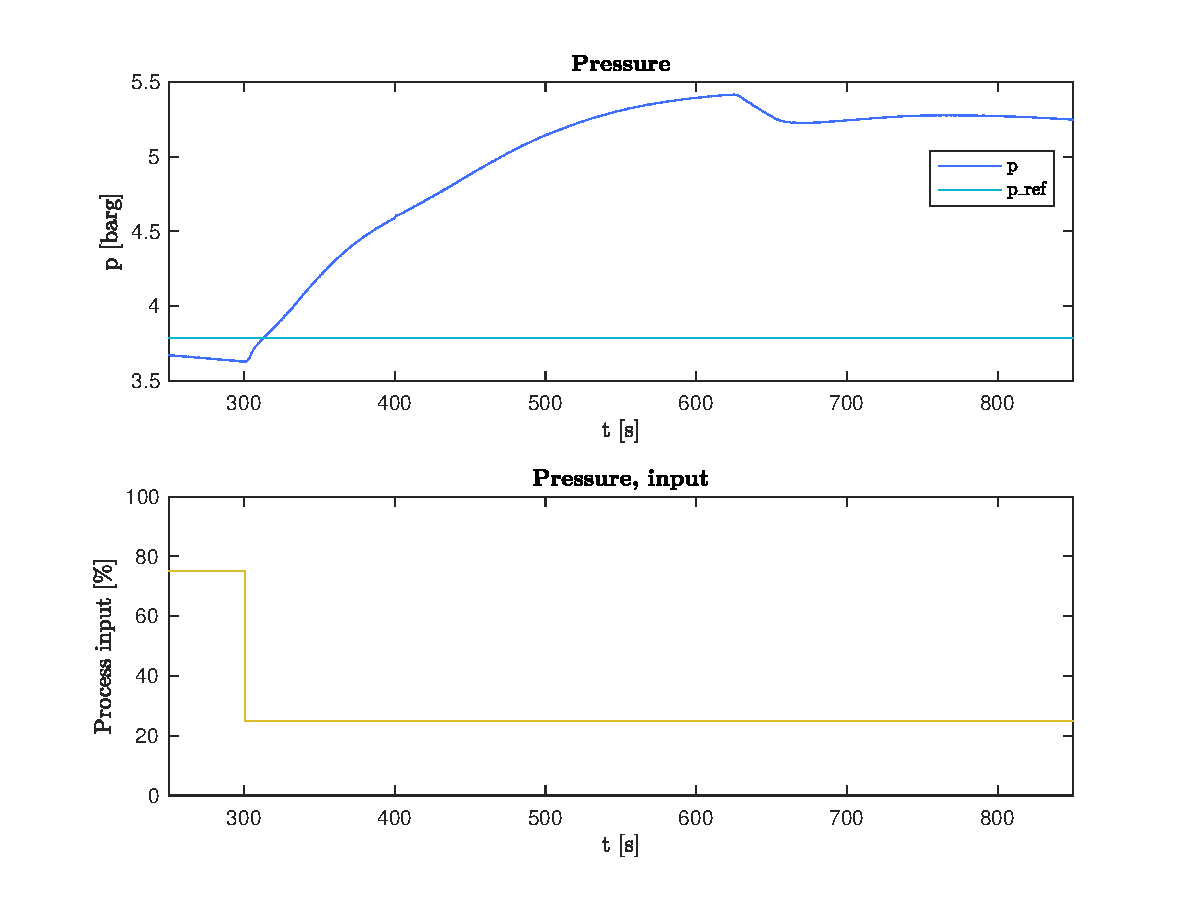
\includegraphics[width=0.8\textwidth]{../Systemanalyse/Log_Data_to_Matlab/Figurer/Stegeksperimenter/PC1024.eps}
\caption{Open-loop step response of $p$}
\label{fig:ol_step_PC1024}

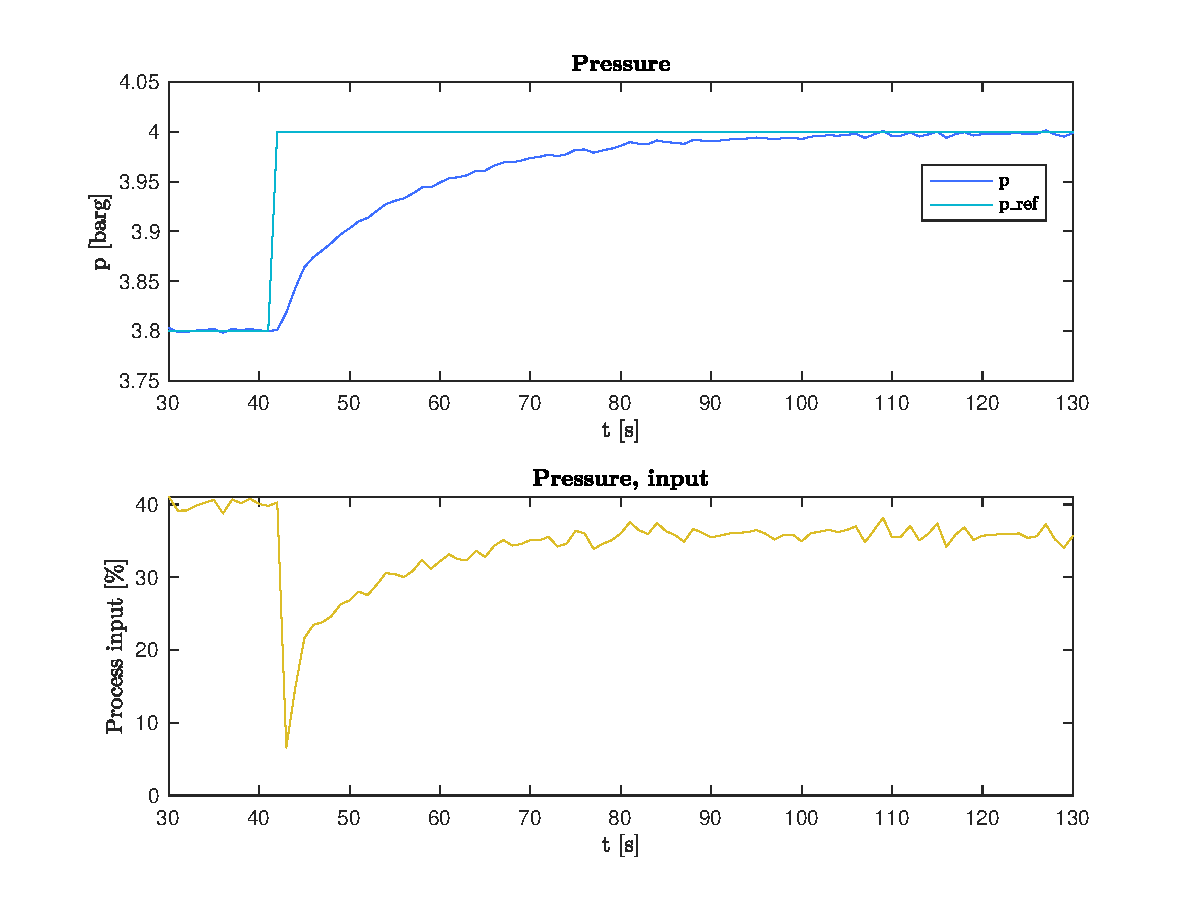
\includegraphics[width=0.8\textwidth]{../Systemanalyse/Log_Data_to_Matlab/Figurer/Stegeksperimenter/PC1024_step.eps}
\caption{Closed-loop step response of $p$}
\label{fig:cl_step_PC1024}
\end{figure}

The step experiments can be seen in figures \ref{fig:ol_step_FC1005}, \ref{fig:ol_step_FC1015}, \ref{fig:ol_step_FC1019}, \ref{fig:ol_step_LC1028} and \ref{fig:ol_step_PC1024}. The reference signals should have been omitted from these plots since we are dealing with open loop systems, and can safely be ignored here.

The plots show that for the first three variables, the accuracy of the simulation is clearly not sufficient for fitting a first order model (they behave in a stepwise fashion). Inspecting the order of magnitude of the gains and time constants may however still be useful. To approximate their sizes, a straight line was drawn from initial state to steady-state.

An attempt at making sense of these parameters is shown in table \ref{tab:inner_loop_step_responses}, together with the fitted values for $V$ and $p$. This gives conservative estimates of $k'$ and $T_1$.

In the table, a desired time constant for the controlled system $T_L$ is shown in the rightmost column. For a quick response, choosing $T_L = 0,3\tau$ is suggested in \cite{balchen}. Some simple trial and error in K-spice showed that this lead to oscillation and unfortunate interaction between control loops, especially the controllers for $D$ and $L$. This is probably partly due to the underestimates of $k'$ and $T_1$ for these variables, since conservative estimates of these results in more aggressive controllers (to compensate for the slow system) when using the SIMC method.

Due to this unsatisfactory behaviour, $T_L = 2\tau$ was chosen for the three fastest control loops instead. The time delay was hard to make a meaningful reading of for the two other systems, so a somewhat arbitrary choice of $T_L = 10s$ was chosen for these systems (instead of using the $T_L = 2\tau$ rule). Like all the other parameters, these were not absolute choices, but a good starting point for further tuning.

After calculating the SIMC controller values some qualitative tuning using K-spice simulations was, not surprisingly, needed. For $D$ and $L$, the integral times were kept fixed, and the gain was decreased to avoid oscillations. For $B$, it was necessary to reduce the integral time in addition to reducing the gain to avoid oscillation. The response of $V$ was slow, and to avoid bandwith limitations in the control of $T_B$ later, both controller parameters were changed to give dramatically more aggressive behaviour. For $p$, the stationary deviation was initially removed pretty slowly, so the integral time was reduced, while also reducing gain to avoid oscillation.

The results of implementing these controllers in K-spice, using the internally scaled gain $G = K_p \frac{(y_{\max} - y_{\min})}{(u_{\max} - u_{\min})}$ for all controllers, are shown in figures \ref{fig:cl_step_FC1005}, \ref{fig:cl_step_FC1015}, \ref{fig:cl_step_FC1019}, \ref{fig:cl_step_LC1028} and \ref{fig:cl_step_PC1024}.


\begin{table}
\centering
\begin{tabular}{c | c | c | c | c | c || c}
& $\tau$ & $T_1$ & $\frac{dy}{dt}$ & $\Delta u$ & $k'$ & $T_L$ \\ \hline
$D$ & 1,0s & 0,4s & 14,3 & 50\% & 28,6 & 2s \\
$L$ & 1,0s & 1,0s & 47,5 & 50\% & 95,0 & 2s \\
$B$ & 1,0s & 0,6s & 10,0 & 50\% & 20,0 & 2s \\
$V$ & $\approx$ 0 & 400s & 0,028 & 20\% & 0,14 & 10s \\
$p$ & $\approx$ 0 & 200s & 0,088 & 50\% & 0,18 & 10s
\end{tabular}
\caption{Identified parameters for inner loop}
\label{tab:inner_loop_step_responses}
\end{table}

\begin{table}
\centering
\begin{tabular}{c | c | c : c | c}
& $K_{p, \textrm{SIMC}}$ & $T_{i, \textrm{SIMC}}$ & $K_{p, \textrm{final}}$ & $T_{i, \textrm{final}}$ \\ \hline
$D$ & 0,012 & 0,4s & 0,0035 & 0,4s\\
$L$ &  0,035 & 1,0s & 0,0018 & 1,0s \\
$B$ & 0,016 & 0,6s & 0,0025 & 1,0s \\
$V$ & 0,71 & 40s & 1,65 & 10s \\
$p$ & 0,57 & 40s & 0,25 & 20s
\end{tabular}
\caption{PI controller parameters for inner loop}
\label{tab:inner_loop_PI_parameters}
\end{table}

\todo{Sørg for å få $p$ skalert riktig (enhet er trykk, ikke flow)}

\newpage
\section{Level controllers}
In this section, the subsystem consisting of the levels in the reflux drum and distillation column is identified, using the inputs $D$ and $B$. Let $y = [M_D \quad M_B]^T$ and $r = [M_{D, \textrm{ref}} \quad M_{B, \textrm{ref}}]^T$. By exciting the controlled system
\begin{equation}
y(s) = L(s)e(s) = G(s) K(s) (y(s) - r(s))
\end{equation}
with changes in the reference $r$, the loop transfer function $L(s) = \frac{y}{e}(s)$ may be identified. Choosing $K(s)$ to be diagonal makes further analysis and controller tuning easier.

\subsection{System identification and analysis}
\subsubsection{Experiment}
The level controllers in the distillation column and reflux drum were expected to be more or less independent, but a MIMO experiment followed by identification using the \texttt{d-sr} toolbox was used anyway, due to the convenience of being able to reuse code in the composition control task. The system was excited by step changes in references for $M_D$ and $M_B$, which were controlled with P controllers, both with $K_p = 1200$. The references were changed after different intervals, to better extract information about all frequencies. The states were attempted held in a reasonable interval, to avoid nonlinear effects such as saturation. The experiments are shown in figures \ref{fig:MD_experiment} and \ref{fig:MB_experiment}.

\subsubsection{Analysis}
The identified model was chosen to have order 2, which is natural for a what was expected to be a diagonal system with two variables. The interactions of the resulting system is shown in figure \ref{fig:BD_RGA}, which show the RGA of the identified $G(s)$. Inspecting this plot shows that the magnitudes of the off-diagonal elements are negligible at frequencies above $10^{-3} \frac{\textrm{rad}}{\textrm{s}}$. The diagonal elements have gain close to unity at the bandwith frequency (which is around $\omega = 0,01$). Since interaction is low, a diagonal controller
\begin{equation}
K(s) =
\begin{bmatrix}
k_1(s) & 0\\
0 & k_2(s)
\end{bmatrix}
\end{equation}
with PI controllers $k_1(s)$ and $k_2(s)$ may be designed independently based on the diagonal elements in the identified $G(s)$. In the following analysis, $L(s)$ is used for simplicity, since it is simply a scaled version of $G(s)$. The controller designed below will then simply be multiplied by the existing $K(s)$ when being implemented.

Figures \ref{fig:L11} and \ref{fig:L22} show the Bode plots of the transfer functions in the diagonals of the identified model. Ignoring the$360^\circ$ error in phase, the gain margin of loop transfer function $l_{11}(s) = \frac{M_D}{M_{D, ref}}(s)$ may be found to be to be 6,74dB as $\omega \rightarrow \infty$. Likewise, the gain margin of $l_{22}(s) = \frac{M_B}{M_{B, ref}}(s)$ is read to be 10,7dB as $\omega \rightarrow \infty$. Using the 6dB gain margin rule of thumb (which is often used in \cite{regtek}), $K_{p, D}$ should not be increased by any significant amount, while $K_{p, B}$ might be increased by a factor of $10^{(10,7-6)/20} \approx 1,7$, yielding the controller gain $K_{p, B} = 2000$.

The phase plot of $l_{11}$ shows that the integral controller should be active in the lower frequency spectrum. To avoid the phase crossing the $-180^\circ$ line, the inequality $\frac{1}{T_{i, D}} < 2 \cdot 10^{-4}$ should be respected. Choosing $T_i = 5000s$ satisfies this. The phase response of $l_{22}$ is pretty similar to the one of $l_{11}$, so initially choosing the same integral time for control of $M_B$ should be reasonable.

Figures \ref{fig:S1} and \ref{fig:S2} shows the magnitudes of the sensitivity functions for the two systems using these controllers. The distillation column is, not surprisingly, the hardest system of the two to control quickly. One might wish to push the bandwith of the $M_B$ loop further to the right, but inspecting the phase plot again suggests not to attempt this. This is because the phase margin would be dangerously low $K_p$ was increased or $T_i$ was decreased, and the system would become more sensitive to time delays and similar phenomena. Disturbances at frequencies above $0,005 \frac{\textrm{rad}}{\textrm{s}}$ should hopefully not be common in this system anyway.

\todo[inline]{Figur av stegrespons til nivåregulering}.

\begin{figure}[p]
\centering
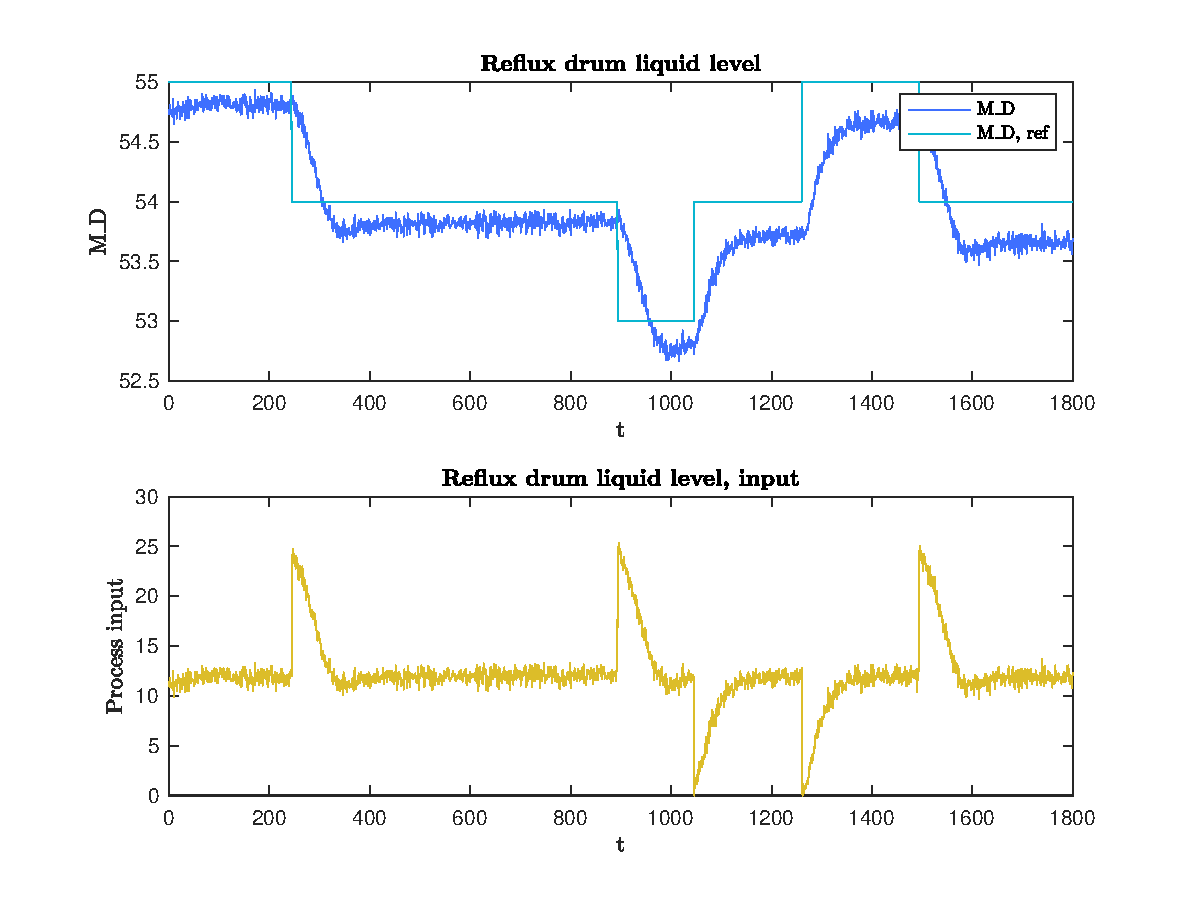
\includegraphics[width=0.8\textwidth]{../Systemanalyse/Log_Data_to_Matlab/Figurer/Identifisering/MD_eksperiment.eps}
\caption{System identification experiment for $M_D$ controller}
\label{fig:MD_experiment}

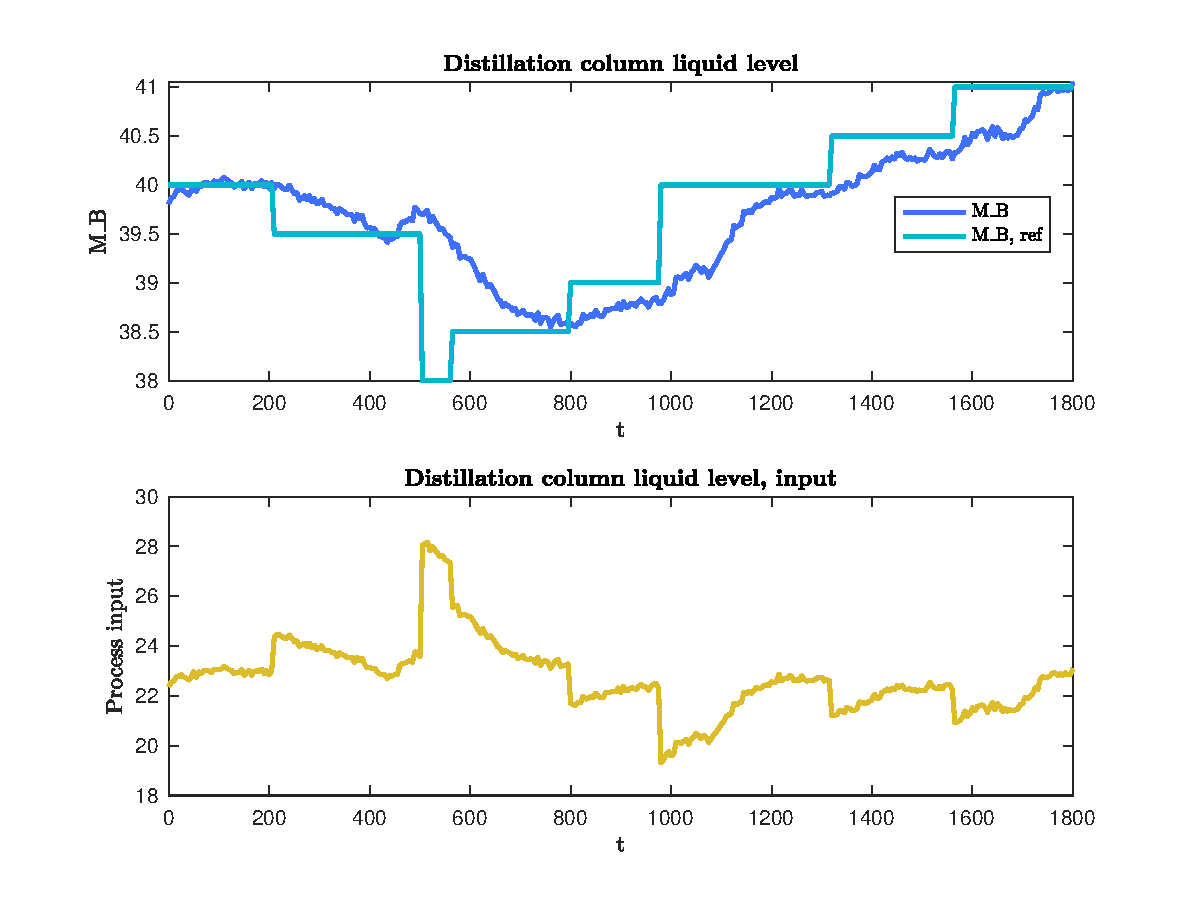
\includegraphics[width=0.8\textwidth]{../Systemanalyse/Log_Data_to_Matlab/Figurer/Identifisering/MB_eksperiment.eps}
\caption{System identification experiment for $M_B$ controller}
\label{fig:MB_experiment}
\end{figure}

\begin{figure}[p]
\centering
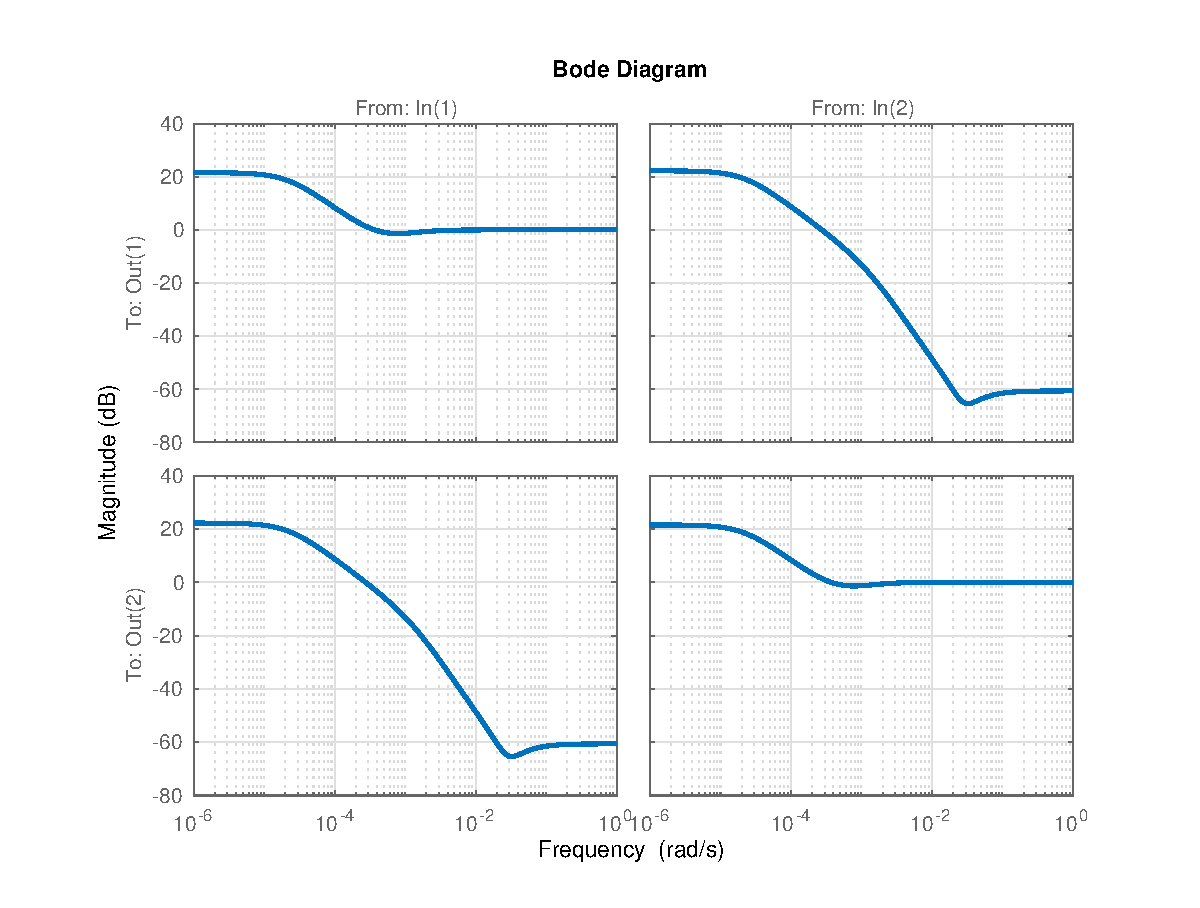
\includegraphics[width=\textwidth]{../Systemanalyse/Log_Data_to_Matlab/Figurer/Identifisering/BD_RGA.eps}
\caption{Magnitude of RGA of identified BD system}
\label{fig:BD_RGA}
\end{figure}

\begin{figure}[p]
\centering
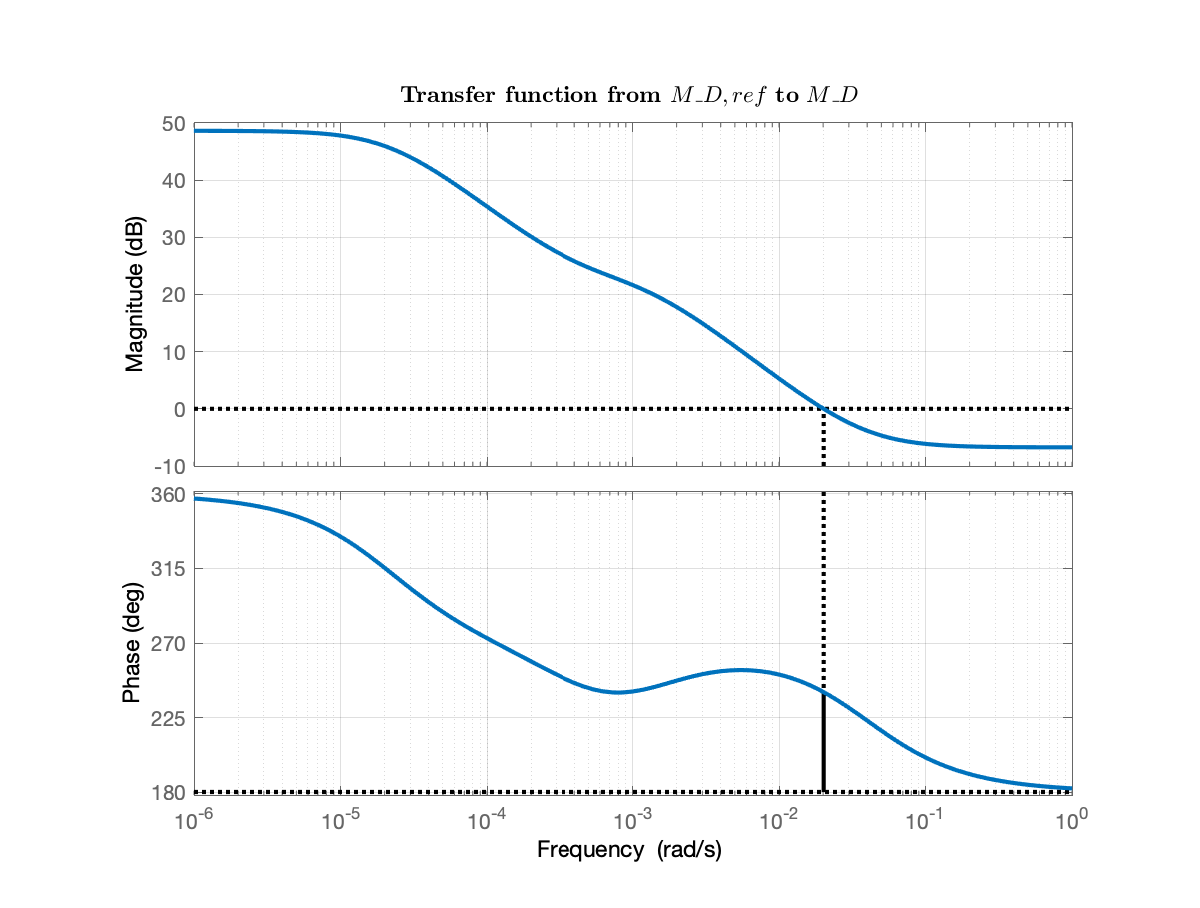
\includegraphics[width=0.8\textwidth]{../Systemanalyse/Log_Data_to_Matlab/Figurer/Identifisering/MD_bode.eps}
\caption{Magnitude and phase response of reflux drum level from reflux drum level reference}
\label{fig:L11}

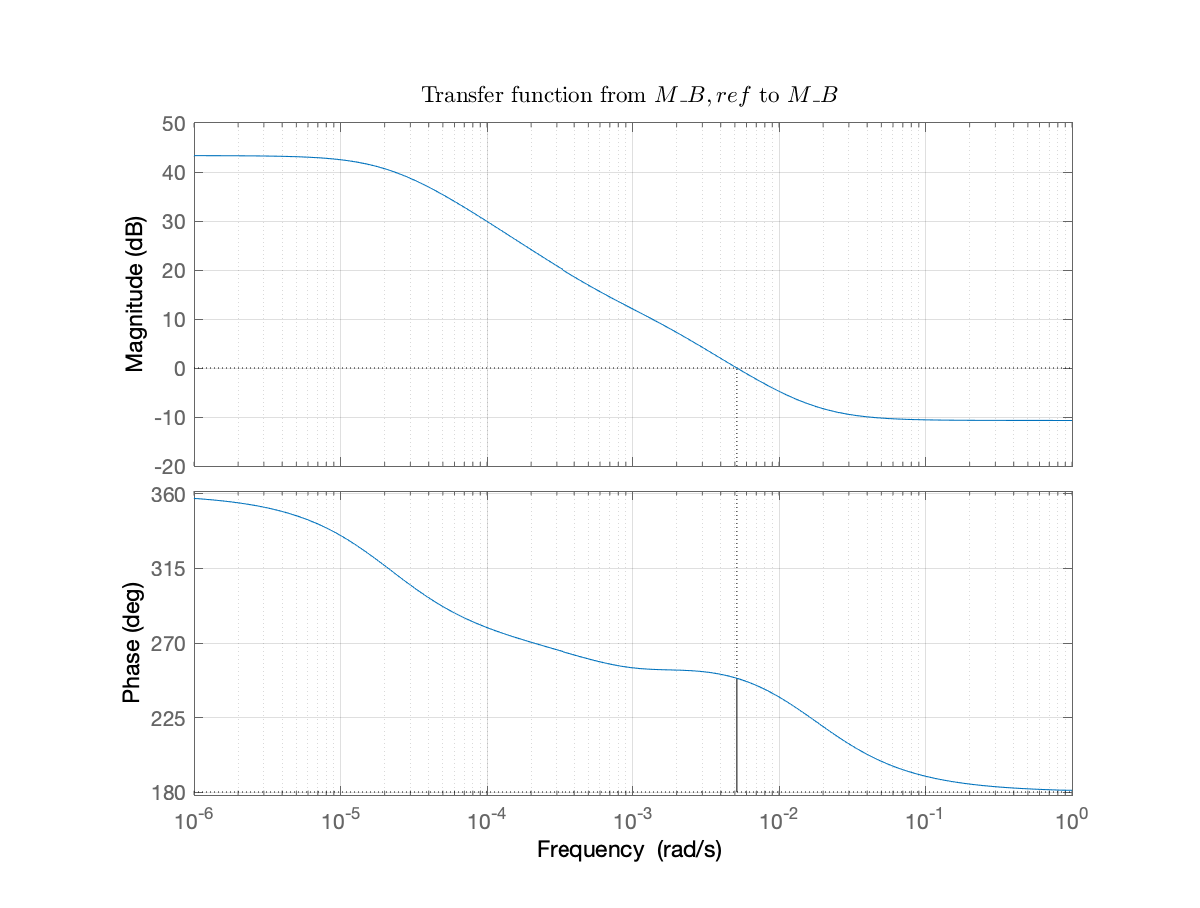
\includegraphics[width=0.8\textwidth]{../Systemanalyse/Log_Data_to_Matlab/Figurer/Identifisering/MB_bode.eps}
\caption{Magnitude and phase response of distillation column level from distillation column level reference}
\label{fig:L22}
\end{figure}

\todo{Dette er teknisk sett transferfunksjon fra feil til tilstand, ikke fra referanse}

\begin{figure}[p]
\centering
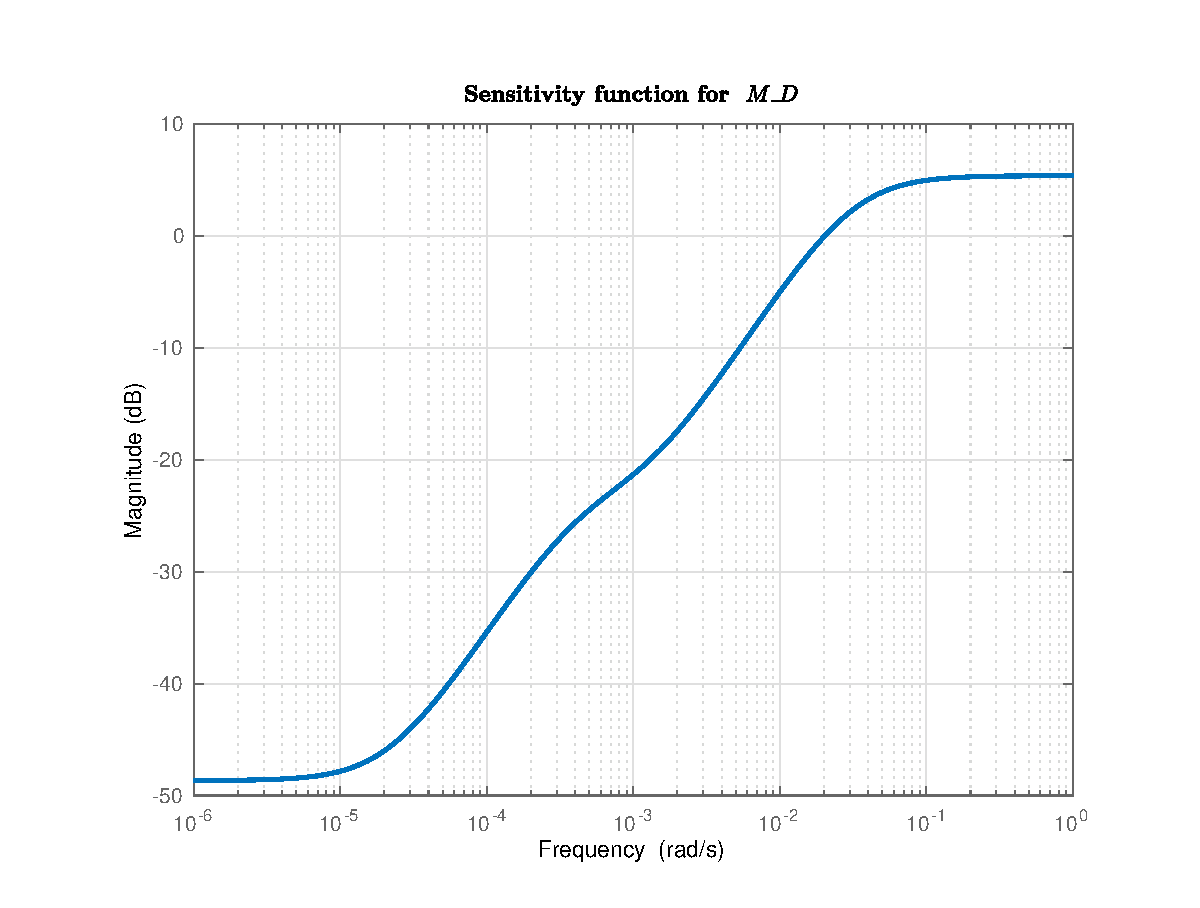
\includegraphics[width=0.8\textwidth]{../Systemanalyse/Log_Data_to_Matlab/Figurer/DB_tuning/S1.eps}
\caption{Sensitivity function for reflux drum level control}
\label{fig:S1}

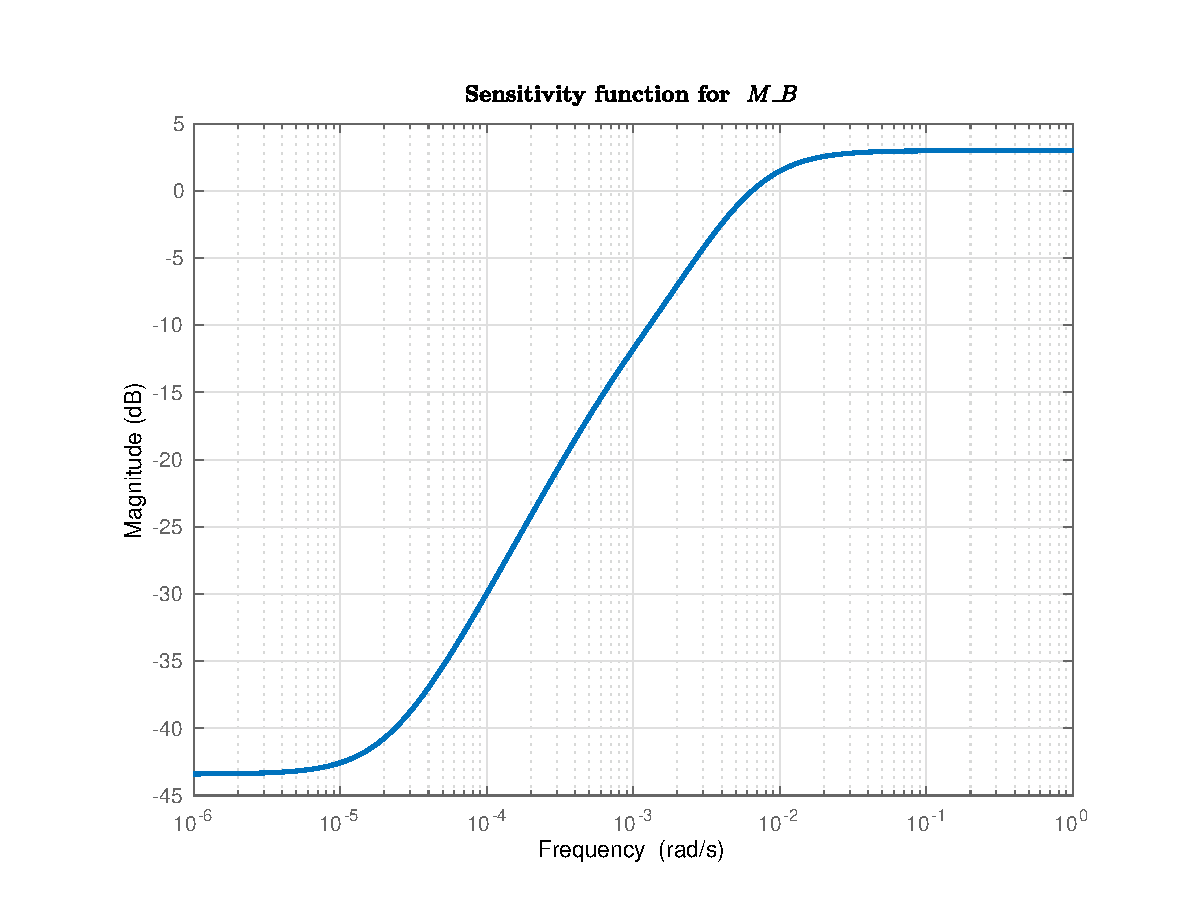
\includegraphics[width=0.8\textwidth]{../Systemanalyse/Log_Data_to_Matlab/Figurer/DB_tuning/S2.eps}
\caption{Sensitivity function for distillation column level control}
\label{fig:S2}
\end{figure}

\subsection{Controller tuning}
Simulation in K-spice showed stationary deviation in $M_D$. To counteract this, the integral time was reduced. Control of $M_B$ worked satisfactory using the PI controller derived from the frequency analysis above.

The initial parameters based on loop-shaping, and the final ones are shown in table \ref{tab:DB_parameters}.

\begin{table}[h]
\centering
\begin{tabular}{c | c | c : c | c}
 & $K_{p, \textrm{initial}}$ & $T_{i, \textrm{initial}}$ & $K_{p, \textrm{final}}$ & $T_{i, \textrm{final}}$\\ \hline
 $M_D$ & 1200 & 5000s & 1200 & 1000s \\
 $M_B$ & 2000 & 5000s & 2000 & 5000s
\end{tabular}
\caption{Parameters for level controllers}
\label{tab:DB_parameters}
\end{table}

\todo{Simulate and plot step responses from K-spice}

\newpage
\section{Composition controllers}
Let $y = [T_D \quad T_B]^T$, $r = [T_{D, \textrm{ref}} \quad T_{B, \textrm{ref}}]^T$ and $u = [L \quad V]^T$. By changing the setpoints for the manipulated variables $L$ and $V$, the system transfer function
\begin{equation}
G(s) = \frac{y}{u}(s)
\end{equation}
may be identified directly.
\subsection{System identification and analysis}
\subsubsection{Experiment}
Identification of the LV system was done in a similar manner as in the previous section, using step changes in input (but open-loop this time). Again, \texttt{d-sr} was used for identification. The periods of the step changes were chosen more systematically than in the level experiment, with periods of 5 minutes, 15 minutes and $\approx2$ minutes being used for different periods of time. This was done to get an accurate representation of the system at all frequencies. The inputs $L$ and $V$ were changed alternatingly (i.e. $90`\circ$ out of phase), to avoid ambiguity in which input caused what effect. Figure \ref{fig:LV_experiment} shows the experiment.

\begin{figure}[p]
\centering
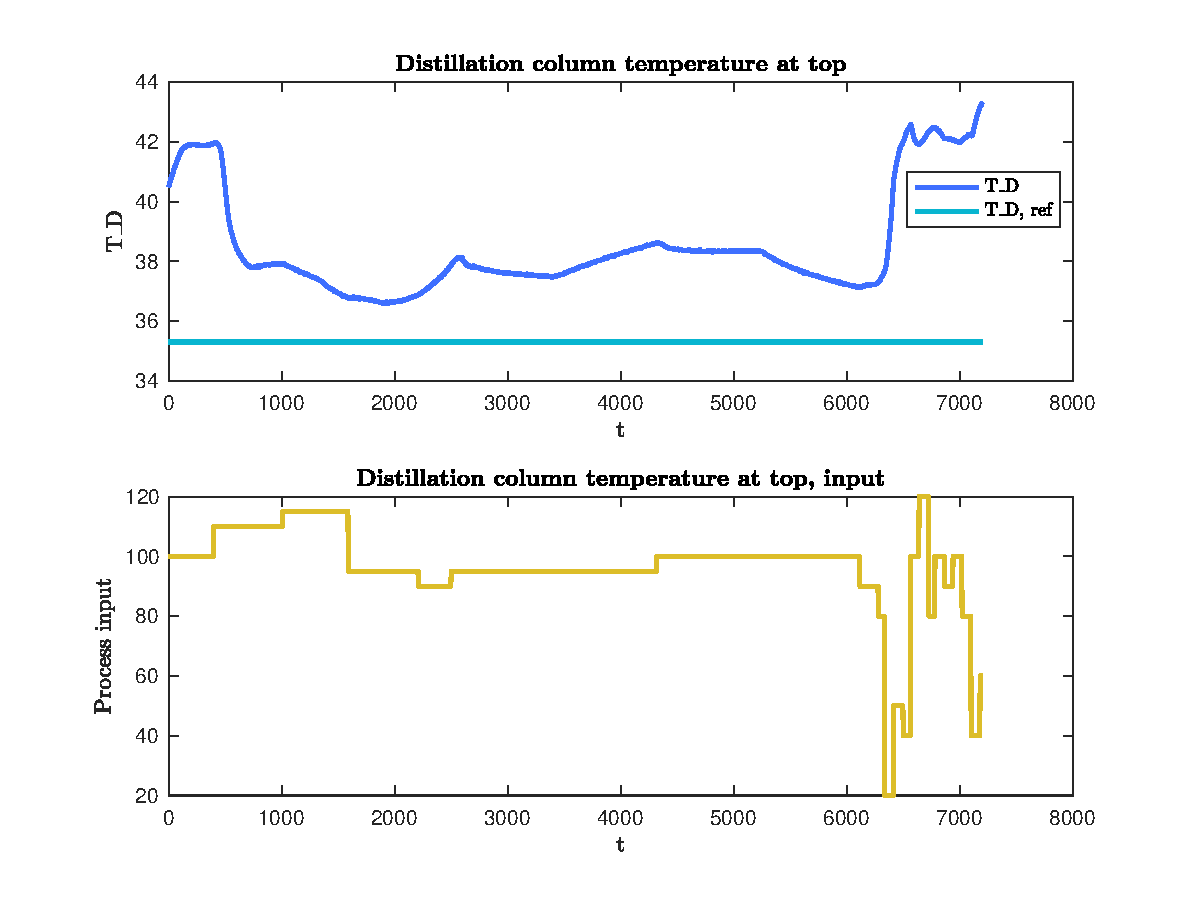
\includegraphics[width=0.8\textwidth]{../Systemanalyse/Log_Data_to_Matlab/Figurer/LV_identifisering/T_D_eksperiment.eps}
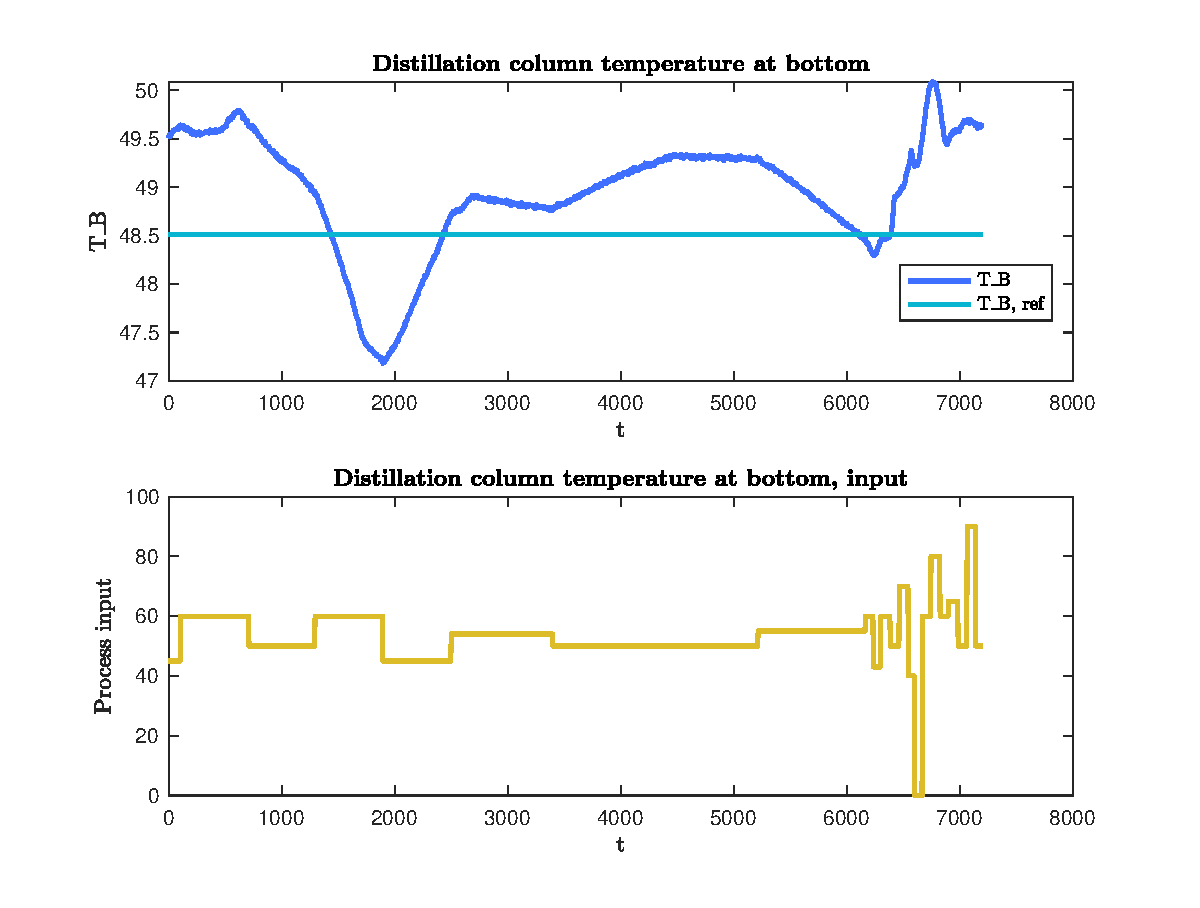
\includegraphics[width=0.8\textwidth]{../Systemanalyse/Log_Data_to_Matlab/Figurer/LV_identifisering/T_B_eksperiment.eps}
\caption{Response of $T_D$ and $T_B $ to step changes in $L$ and $V$}
\label{fig:LV_experiment}
\end{figure}

\subsubsection{Analysis}
Figure \ref{fig:LV_RGA} shows the RGA of the identified system $G(s) = \frac{y}{u}(s)$. The chosen pairing is clearly the most reasonable. The interactions doesn't seem to be too severe, but the RGA doesn't tell the whole story. It should seem reasonable that temperature in the bottom affects temperature in the top more than the other way around, and the right tool for this analysis is the \textit{Performance Relative Gain Array} (PRGA). To use this however, the system has to be rescaled.

More precisely, given a system

\begin{equation}
e = y - r = G(s) u + G_d(s) d - r
\end{equation}
the signals should be scaled such that the maximum disturbance and maximum acceptable error both are of magnitude less than one. Table \ref{tab:LV_scaling} shows the range used in K-spice for the states, and maximum value for signals only used in analysis. To be clear, the following analysis holds for both control loops, with $y$ being temperature, $r$ reference temperature, and $u$ process input. The maximum error allowed is chosen based on the lowest margin proposed in the assignment text. The choice of one degree celsius is somewhat arbitrary, but seemed reasonable and at least not too optimistic given the information that one degree is considered a large step.

The PRGA using this scaling is shown in figure \ref{fig:LV_PRGA}. It is now clear that one can't simply choose a bandwith of $0,01 \frac{\textrm{rad}}{\textrm{s}}$ and call it a day, since the interaction from $V$ to $T_D$ has its peak at this frequency.



\begin{table}
\centering
\begin{tabular}{c | c | c | c}
Variable & Min & Max & Maximum magnitude \\ \hline
$T_D$ & $25^\circ$C & $50^\circ$C & $25^\circ$C \\
$T_B$ & $25^\circ$C & $50^\circ$C & $25^\circ$C \\
$T_{D, \textrm{ref}}$ & $25^\circ$C & $50^\circ$C & $25^\circ$C \\
$T_{B, \textrm{ref}}$ & $25^\circ$C & $50^\circ$C & $25^\circ$C \\
$L$ & $0 \frac{\textrm{t}}{\textrm{h}}$ & $120 \frac{\textrm{t}}{\textrm{h}}$ & $120 \frac{\textrm{t}}{\textrm{h}}$ \\
$V$ & $0\%$ & $100\%$ & $100\%$ \\
$e$ & - & - & $0,55^\circ$C \\
$d$ & - & - & $1,0^\circ$C
\end{tabular}
\caption{Scaling used in LV system analysus}
\end{table}

\begin{figure}[p]
\centering
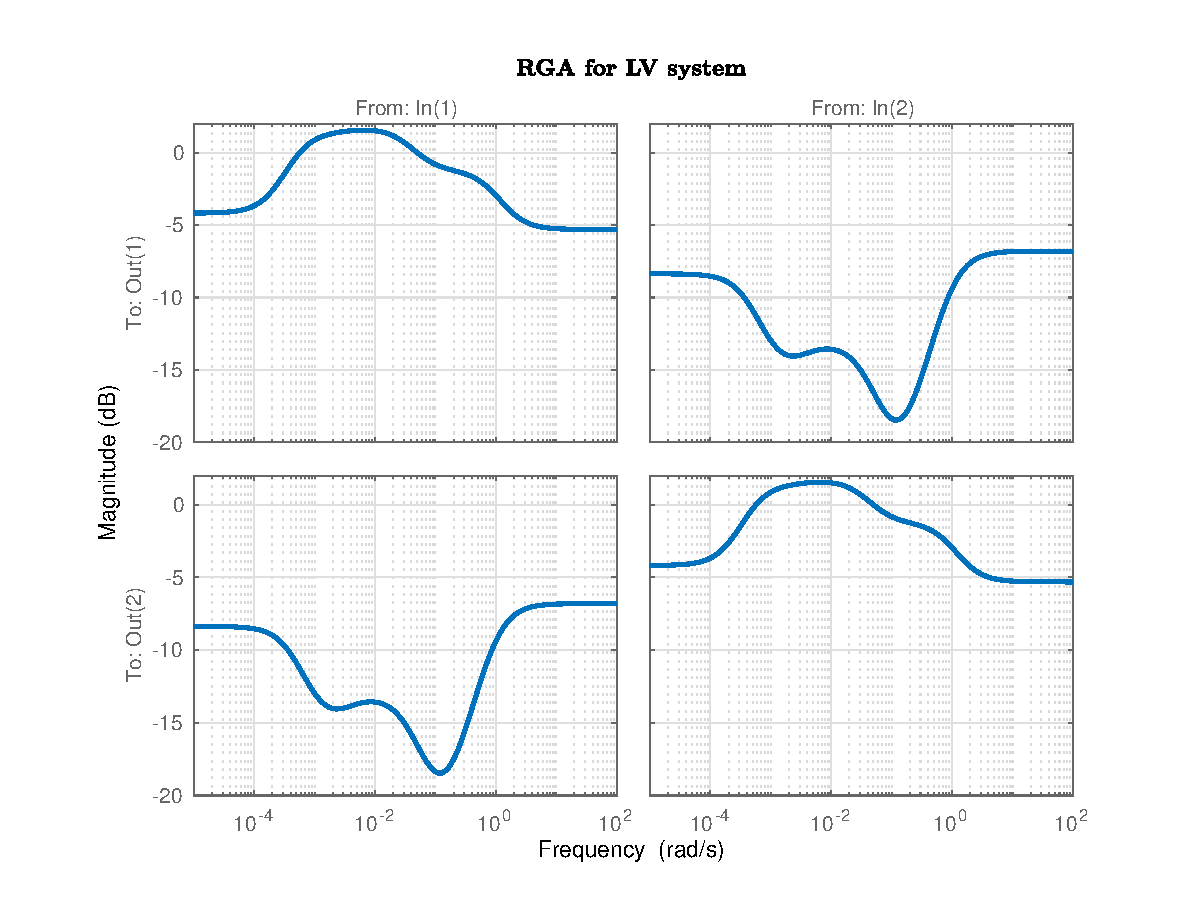
\includegraphics[width=0.8\textwidth]{../Systemanalyse/Log_Data_to_Matlab/Figurer/LV_identifisering/LV_RGA.eps}
\caption{RGA for LV system}
\label{fig:LV_RGA}
\end{figure}

\begin{figure}[p]
\centering
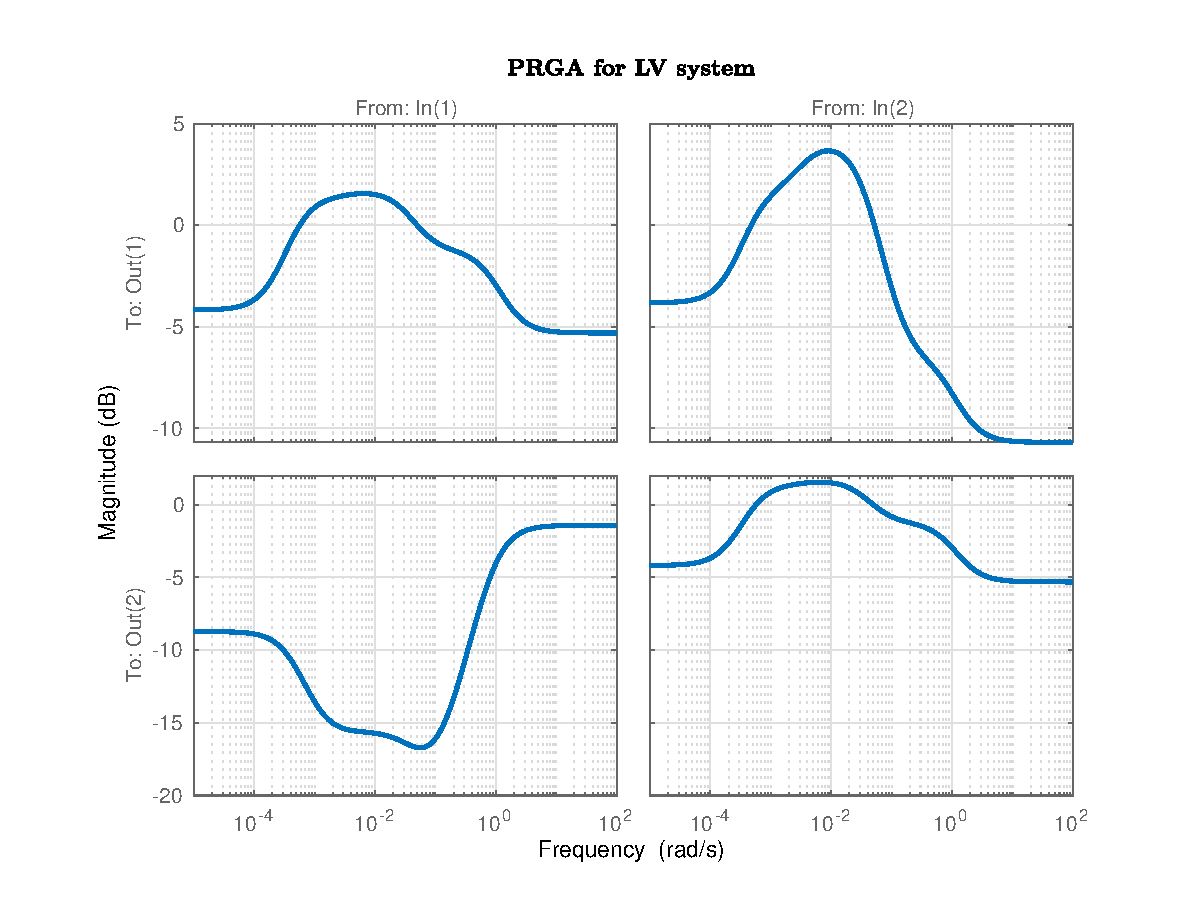
\includegraphics[width=0.8\textwidth]{../Systemanalyse/Log_Data_to_Matlab/Figurer/LV_identifisering/LV_PRGA.eps}
\caption{PRGA for LV system}
\label{fig:LV_PRGA}
\end{figure}

\subsection{Controller tuning}
\todo[inline]{Tune i K-spice}


\newpage
\section{Results}
\subsection{PI controller tuning}
Table \ref{tab:final_controller_parameters} shows the final PI controller parameters for all the control loops tuned in this project, also including the scaled gain $G$ used in the K-spice implementation.

\begin{table}
\centering
\begin{tabular}{c | c | c | c }
& $K_p$ & $G$ & $T_i$ \\ \hline
$D$ (FC1005) & 0,0035 & 0,42& 0,4s\\
$L$ (FC1015) & 0,0018 & 0,22 & 1,0s \\
$B$ (FC1019) & 0,0025 & 0,3 & 1,0s \\
$V$ (LC1028) & 200 & 200 & 10s \\
$p$ (PC1024) & 5 & 30 & 20s \\
$M_D$ (LC1016) & 1200 & 10 & 1000s \\
$M_B$ (LC1015) & 2000 & 16,7 & 5000s \\
$T_D$ (TC1015) & 12 & 2,5 & 100s \\
$T_B$ (TC1088) & 25 & 6,3 & 1000s
\end{tabular}
\caption{Final controller parameters}
\label{tab:final_controller_parameters}
\end{table}

\subsection{Reference tracking}
The results of step changes in reference are shown in figures \ref{fig:T_D_step} and \ref{fig:T_B_step}.

\begin{figure}
\centering
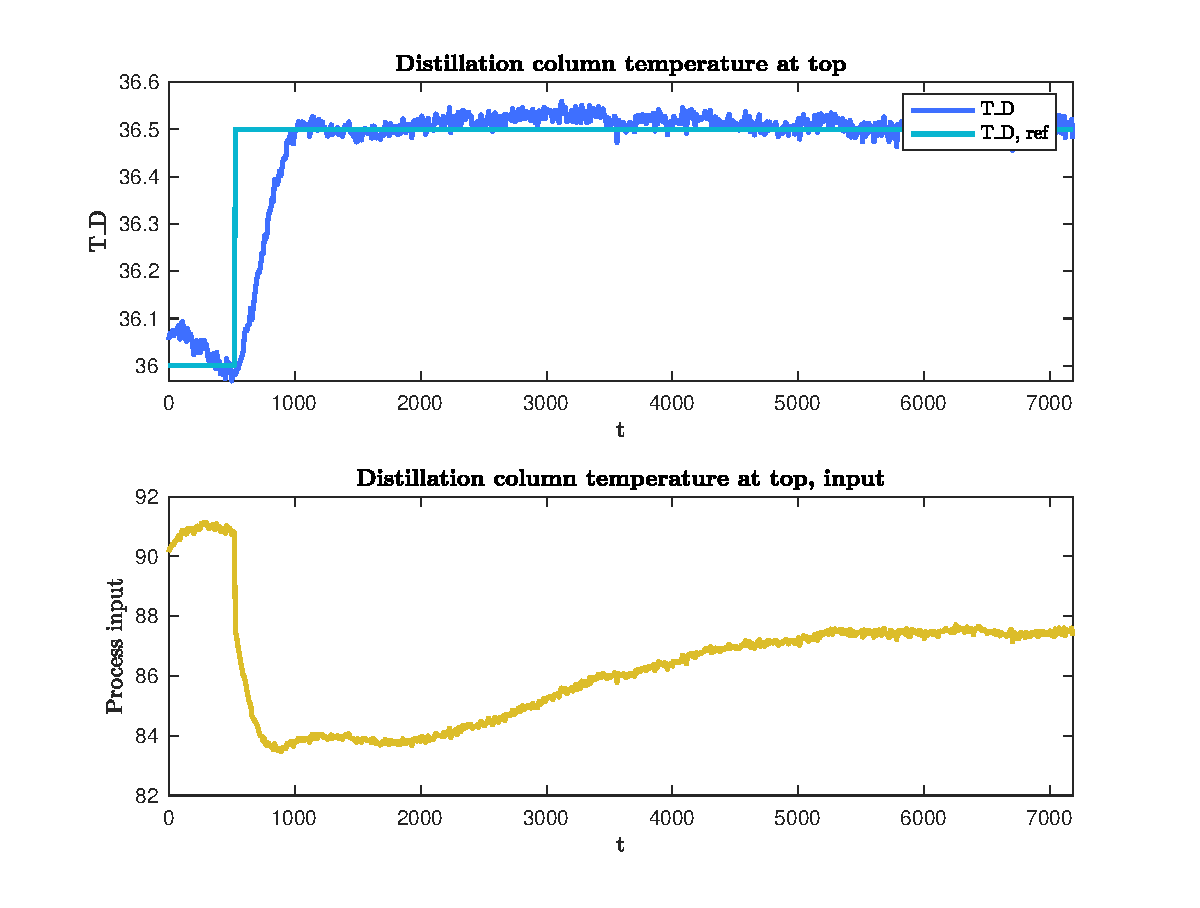
\includegraphics[width=0.8\textwidth]{../Systemanalyse/Log_Data_to_Matlab/Figurer/LV_tuning/T_D_with_T_D_step.eps}
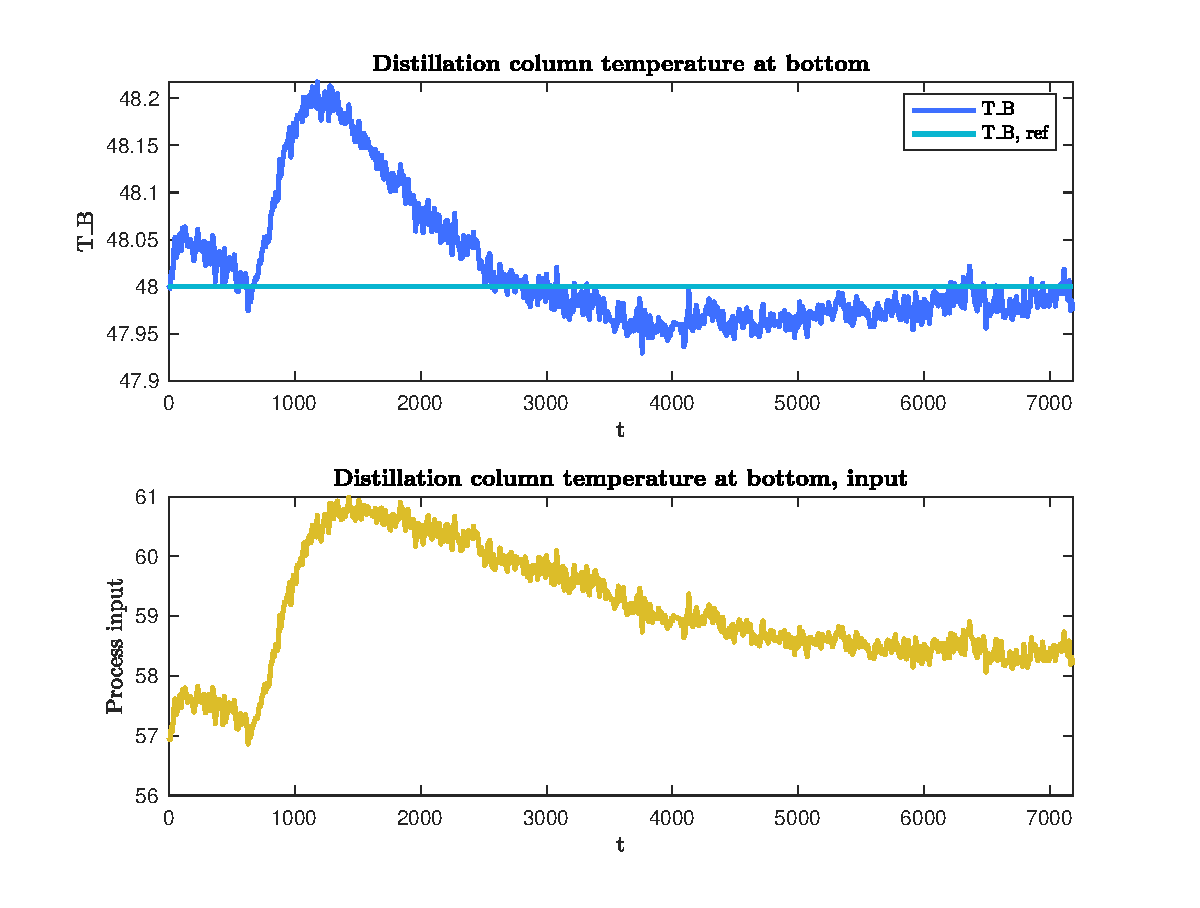
\includegraphics[width=0.8\textwidth]{../Systemanalyse/Log_Data_to_Matlab/Figurer/LV_tuning/T_B_with_T_D_step.eps}
\caption{Response of $T_D$ and $T_B $ to step change in $T_{D, \textrm{ref}}$}
\label{fig:T_D_step}
\end{figure}

\begin{figure}
\centering
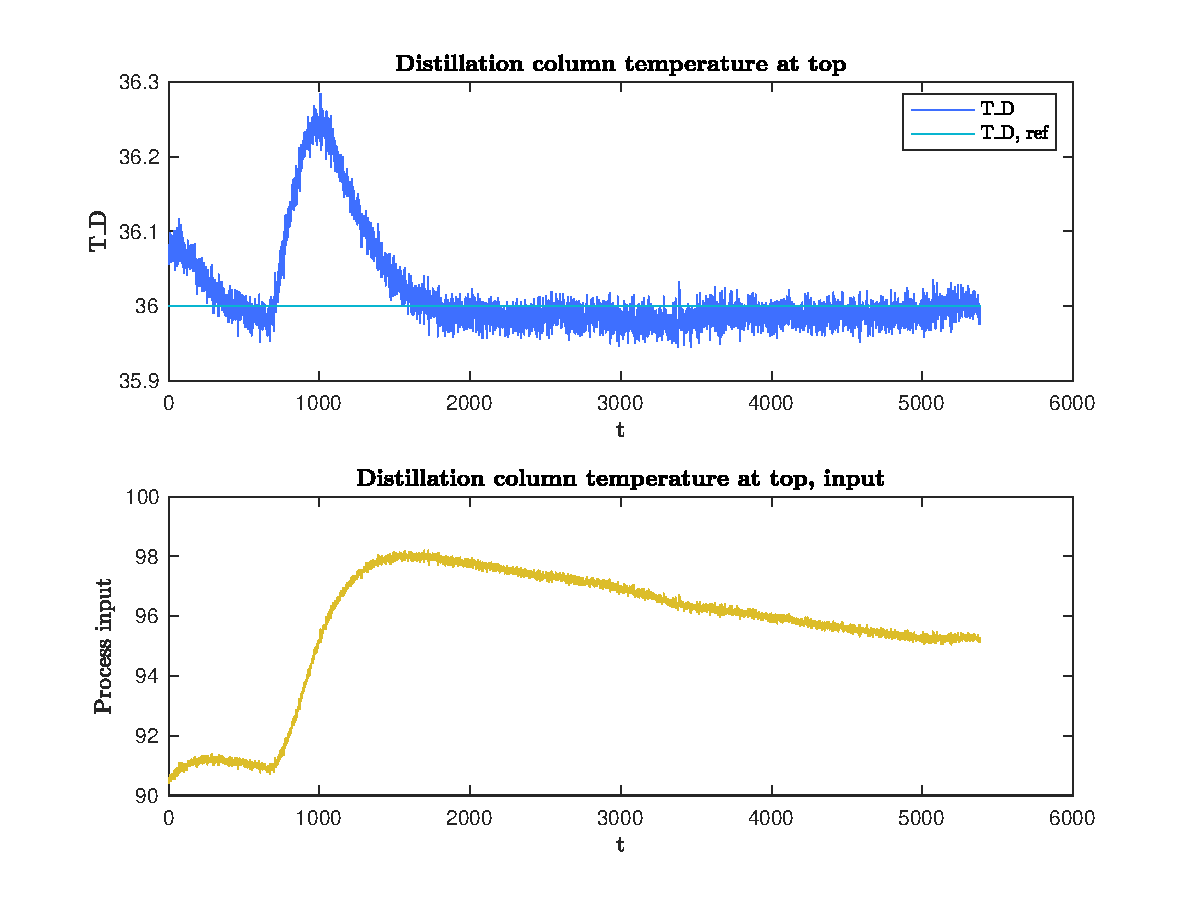
\includegraphics[width=0.8\textwidth]{../Systemanalyse/Log_Data_to_Matlab/Figurer/LV_tuning/T_D_with_T_B_step.eps}
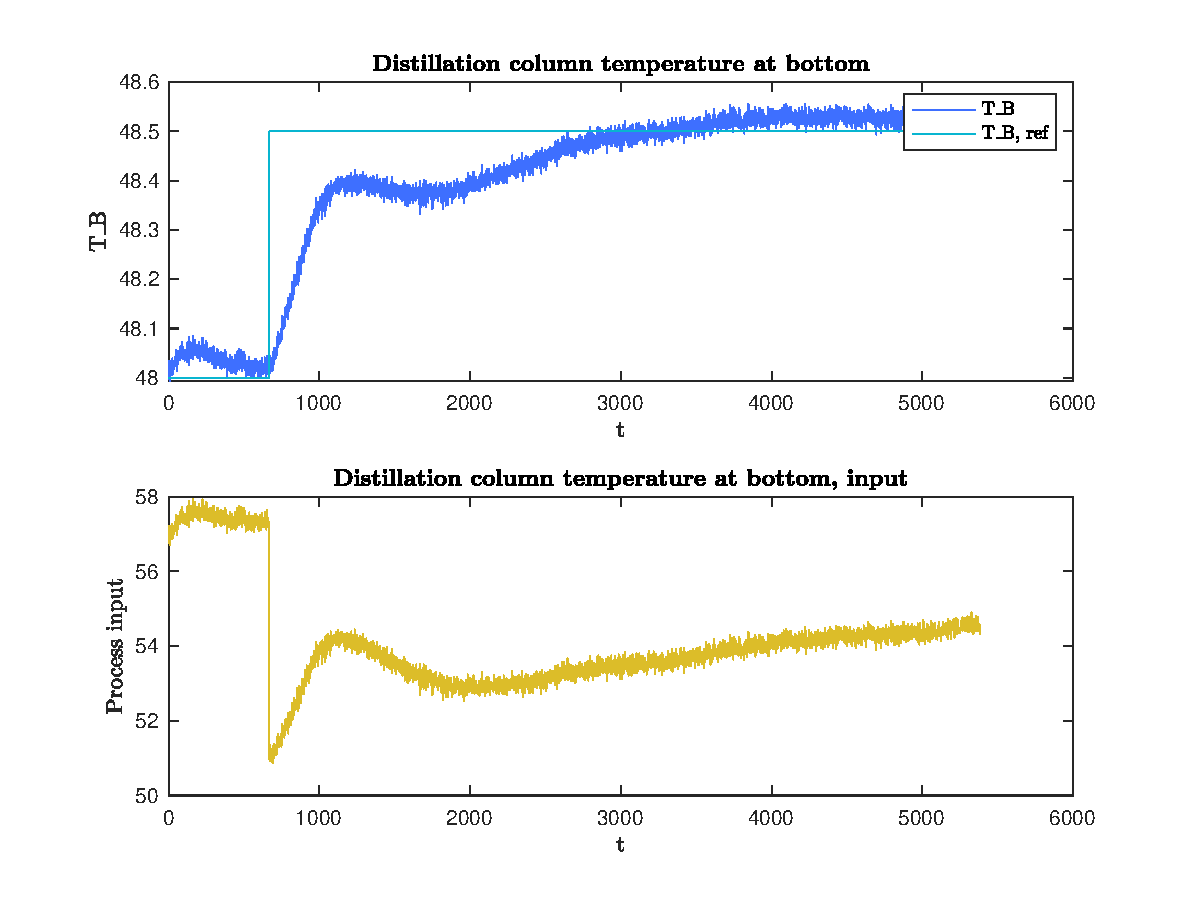
\includegraphics[width=0.8\textwidth]{../Systemanalyse/Log_Data_to_Matlab/Figurer/LV_tuning/T_B_with_T_B_step.eps}
\caption{Response of $T_D$ and $T_B $ to step change in $T_{B, \textrm{ref}}$}
\label{fig:T_B_step}
\end{figure}

\newpage
\begin{thebibliography}{9}

\bibitem{oppgavetekst}
  Morten Hovd,
  \textit{TTK4210 Advanced Control of Industrial Processes, Assignment 6},
  2020.

\bibitem{skogestad}
  Sigurd Skogestad and Ian Postlethwaite,
  \textit{Multivariable Feedback Control},
  John Wiley \& Sons Ltd, Chichester,
  2nd edition,
  2005.
  
\bibitem{regtek}
  Jens G. Balchen, Trond Andresen and Bjarne A. Foss,
  \textit{Reguleringsteknikk},
  Institutt for Teknisk Kybernetikk, Trondheim,
  6th edition,
  2016.

\end{thebibliography}

\end{document}
